
    \section{Gestione della Memoria}
    La memoria é oggi a basso costo, e con trend in diminuzione, questo fa si che le applicazioni usino sempre piú memoria,
    se ogni processo dovesse gestire la propia memoria, ogni processo userebbe semplicemente tutta la memoria disponibile,
    questo porterebbe all'assenza della multiprogrammazzione che é un aspetto essenziale per il corretto funzionamento del
    sistema operativo, si potrebbe imporre dei limiti di memoria a ciascun processo, diventa peró difficile per un programmatore
    scrivere un processo che rispetti tali limiti, quindi ogni sistema operativo deve avere un sistema di gestione della memoria
    cercando di dare l'illusione ai processi di avere tutta la memoria, la soluzione é quella di usare il disco come buffer
    per memoria, questa gestione di I/O é ovviamente piú lenta del processore, per cui il SO deve pianificare lo swap
    \subsection{Requisiti}
    \begin{itemize}
        \item Rilocazione : importante che ci sia aiuto hardware, aiuto, non gestione diretta per cui sistema operativo e hardware collaborano
        \item Protezione : importante che ci sia un aiuto hardware
        \item Condivisione
        \item Organizzazione logica
        \item Organizzazione fisica
    \end{itemize}
    \subsubsection{Rilocazione}
    Il programmatore non sa e non deve sapere in quale zona della memoria il programma verrá caricato :
    \begin{itemize}
        \item potrebbe essere swappato su disco, e al ritorno in memoria principale potrebbe essere caricato in un'altra zona
        \item potrebbe anche non essere contiguo, oppure con altre pagine in RAM e altre in disco
        \item in questo contesto, si intende chi usa l'assembler o il compilatore
    \end{itemize}
    I riferimente alla memoria devono essere tradotti nell'indirizzo fisico : preprocessing, run-time,se run-time occrre supporto hardware
    \begin{figure}[H]
        \centering
        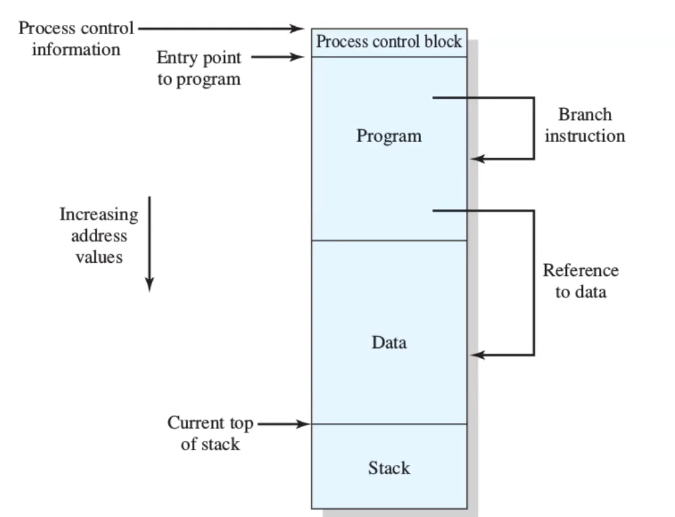
\includegraphics[width=0.75\textwidth]{immagini/RilocazioneIndirizziNeiProgrammi}
        \caption{Rilocazione}
    \end{figure}
    un processo ha una zona con il programma in liguaggio macchina, e una zona con i dati, e una zona con lo stack, la sua parte iniziale
    é il PCB, gli indirizzi che possiamo avere sono indirizzi di salto oppure referenze a variabili, tutti questi inidirizzi
    devono essere ricalcolati.
    \subsubsection*{Indirizzi nei programmi}
    \begin{figure}[H]
        \centering
        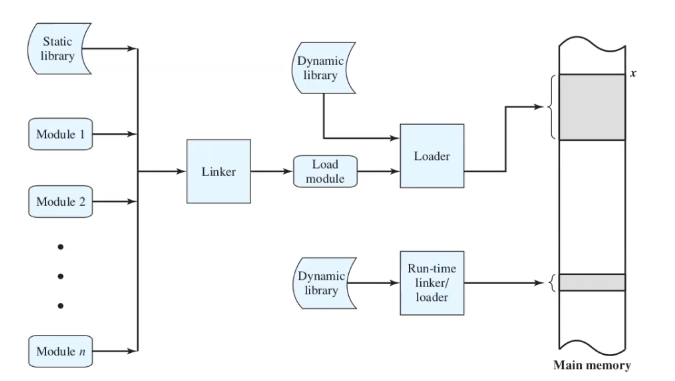
\includegraphics[width=0.75\textwidth]{immagini/Indirizzi nei programmi}
        \caption{Indirizzi nei programmi}
    \end{figure}
    Per capire come avviene la rilocazione dobbiamo prima precisare... Un programma eseguibile viene prima scritto
    in moduli, uno di questi moduli ha il main, quindi ci sono tanti moduli scritti dal programmatore oppure librerie
    , ognuno di questi moduli viene compilato separatamente, ed per ogni modulo viene creato un file oggetto, tutto
    questo viene collegato attraverso il linker in modo da creare un file eseguibiler (nell'esempio Load module),
    poi c'é il loader che carica il file eseguibile in memoria, nel fare questo ci potrebbe essere bisogno di alcune librerie dinamiche
    \begin{figure}[H]
        \centering
        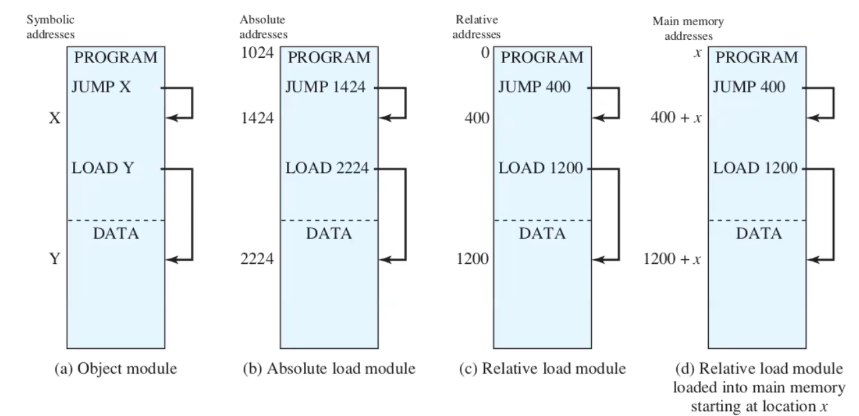
\includegraphics[width=0.75\textwidth]{immagini/IndirizziInMemoria}
        \caption{Effettivo in memoria}
    \end{figure}
    Il risultato é mostrato nell'immagine, ogni singolo modulo ha la sua parte di programma e la sua parte di dati,
    sostanzialmente il programma contiene soltanto indirizzi simbolici, quando peró viene trasformato in un file eseguibile
    abbiamo 2 possibilitá:
    \begin{itemize}
        \item Indirizzo Assoluto : Lui sa che deve cominciare a 1024, e se deve saltare a 1424, il loader deve caricare il programma all'indirizzo 1024 altrimenti non funziona.
        \item Indirizzo Relativo : Con gli inderizzi relativi, si puó suppore di partire da 0, e nel caso di un salto scrivo solo l'indirizzo rispetto all'inizio del programma.
    \end{itemize}
    \subsubsection*{Tipi di Indirizzi}
    \begin{itemize}
        \item \textbf{Indirizzi Logici} : vengono usati dal programmatore, sono indirizzi simbolici, non sono reali, sono rilocati
        \item \textbf{Indirizzi Fisici} : sono gli indirizzi reali, sono quelli che vengono usati dal processore
        \item \textbf{Indirizzi Relativi} : il riferimento é espresso come un un spiazzamento rispetto ad un punto di riferimento.
    \end{itemize}
    \begin{figure}[H]
        \centering
        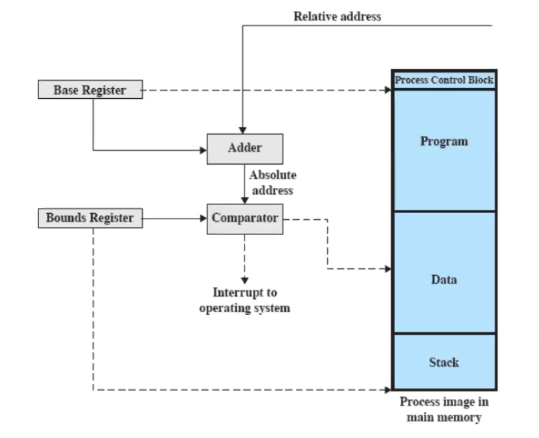
\includegraphics[width=0.75\textwidth]{immagini/RilocazioneConHardware}
        \caption{Tipi di Indirizzi}
    \end{figure}
    Nel caso di indirizzi relativi, l' hardware della macchina sa che se per esempio abbiamo un salto a 100, allora
    l'hardware sa che deve sommare 100 all'indirizzo base (Es. 6000), quindi l'indirizzo fisico sará 6100, inoltre c'é una
    fase di controllo per rimanere nei limiti di memoria, e fondamentale che ogni volta che il sistema operativo carica il
    processo il sistema operativo deve preoccuparsi di mettere l'indirizzo corretto nel base register.\\

    I registri usati sono:
    \begin{itemize}
        \item Base Register : contiene l'indirizzo base del processo.
        \item Limit Register : contiene l'indirizzo di fine del processo.
    \end{itemize}
    I valori per questi registri vengono settati nel momento in cui il processo viene posizionato in memoria, mantenuti nel PCB del processo,
    fa parte del passo 6 del process switch e non vanno semplicemente modificati occore propio modificarli.
    \subsubsection{Protezione}
    I processi non devono poter accedere alla locazione di memoria di memoria di un'altro processo, a meno che
    non sia stato esplicitamente condiviso, A causa della rilocazione non puó essere fatto a tempo di compilazione,
    pertanto serve un supporto hardware.
    \subsubsection{Condivisione}
    La condivisione deve essere possibile, permettere a piú processi di accedere alla stessa locazione di memoria, solo se é effettivamente
    utile allo scopo perseguito, c'é anche casi in cui é il sistema operativo in maniera trasparente, il caso tipico é quando
    si seseguono piú processi eseguendo lo stesso codice sorgente, quindi lo metto in RAM una volta sola.
    \subsubsection{Organizzazione Logica}
    A livello hardware, la memoria é organizzata in modo lineare, A livello software , i programmi sono scritti in moduli,
    per cui il SO deve offrire tali caratteristiche, facendo da ponte tra la prima visuale (moduli) e la seconda (lineare).
    \subsubsection{Organizzazione Fisica}
    L' organizzazione fisica é quella che si occupa del flusso di dati tra RAM e la memoria secondari, questa non é una
    cosa lasciata al programmatore, se per esempio io scrivo un programma che necessitá di 1GB di ram ma il sistema
    operativo me ne assegna 500MB, una volta il programmatore doveva usare l'overlay per suddividere il programma in
    pezzi e gestire lo swap tra ram e disco in maniera manuale, oggi il sistema operativo si occupa di tutto ció.
    \subsection{Partizionamento}
    Uno dei primi metodi per gestire la memoria é il partizionamento, la memoria viene divisa in partizioni, esso
    puó essere di diversi tipi:
    \begin{itemize}
        \item \textbf{Partizionamento Fisso} : la memoria é divisa in partizioni di dimensione fissa.
        \item \textbf{Partizionamento Dinamico} : la memoria é divisa in partizioni di dimensione variabile.
        \item \textbf{Paginazione Semplice} : la memoria é divisa in pagine di dimensione fissa.
        \item \textbf{Segmentazione Semplice} :
        \item \textbf{Paginazione con memoria virtuale} :
        \item \textbf{Segmentazione con memoria virtuale} :
    \end{itemize}
    \subsubsection{Partizionamento Fisso Uniforme}
    Quando accendo il sistema operativo, tra le cose che vengono fatte il SO divide la memoria in partizioni di dimensione
    fissa, 1 é riservata al kernel, le altre sono per i processi, l'idea é quella di mettere al loro interno i processi
    che peró non possono superare la partizione assegnata all'inizio, chiaramente il SO puó decidere se sospendere
    e quindi spostare il processo sul disco, in questo caso era il programmatore a dover essere sicuro di non sforare
    la partizione assegnata.
    \subsubsection*{Problemi}
    un programma potrebbe non entrare in una partizione, questo porta anche ad un uso inefficiente della memoria, perché
    porta al fenomeno della frammentazione interna.
    \subsubsection{Partizionamento Fisso Variabile}
    Nel partizionamento variabile comunque le partizioni vengono assegnate una sola volta, ma la dimensione delle partizioni
    é variabile, questo permette di mettere i processi piú leggeri in partizioni piú piccole.
    \subsubsection*{ALgoritmo di Posizionamento}
    Da momento in cui ho partizioni di dimensioni variabili, mi devo preoccupare di dove mettere i processi, una scelta
    é quella di avere una coda per partizione , oppure ho una unica coda e mano a mano assegno alla partizione che spreca
    meno spazio, se uso la coda unica posso fare delle ottimizzazioni nel senso che piuttosto che non far eseguire un
    processo lo carico in memoria, anche se spreco un po' di memoria.
    \begin{figure}[H]
        \centering
        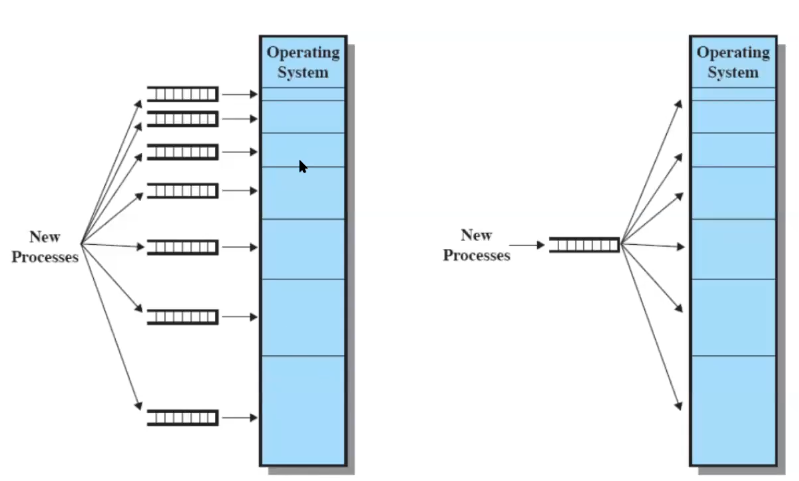
\includegraphics[width=0.75\textwidth]{immagini/partizionamento}
        \caption{Partizionamento Variabile}
    \end{figure}
    \subsubsection*{Problemi Irrisolti}
    C'é un numero massimo di processi in memoria principale dettato dal fatto che il numero di processi non puó superare
    il numero di partizione, inoltre la gestione della memoria risulta comunque inefficiente se ho tanti processi piccoli.
    \subsubsection{Partizionamento Dinamico}
    Le partizioni variano sia in misura che in quantitá, la dimensione delle partizione varia in base alla dimensione 
    del processo.
    \subsubsection*{Esempio}
    \begin{figure}
        \centering
        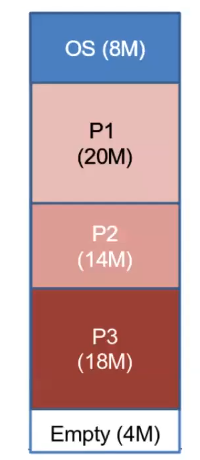
\includegraphics[width=0.75\textwidth]{immagini/EsempioPartizionamentoDinamico}
        \caption{Partizionamento Dinamico}
    \end{figure}
    Supponiamo che arrivino in sequenza tre processi, p1=20MB, p2=14MB, p3=18MB, stiamo
    assumendo che chiaramente stiamo usando indirizzi relativi, in una memoria da 56M
    resta un blocco da 4MB, se arriva un processo da 5MB, il sistema operativo deve fare una
    scelta, supponiamo che il processo da 5MB sia il processo p4 e sia piú importante di p2
    \begin{figure}[H]
        \centering
        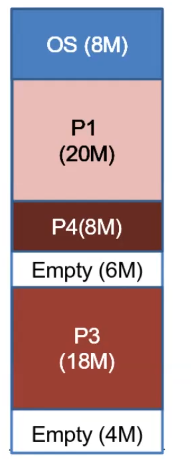
\includegraphics[width=0.75\textwidth]{immagini/EsempioPartizionamentoDinamico2}
        \caption{Partizionamento Dinamico}
    \end{figure}
    quello che succede é che si lascia uno spazio vuoto di 6MB, p2 chiaramente viene copiato
    sul disco in attesa che venga richiamato, ora peró vogliamo far eseguire p2 che é piú importante
    di p1 copiamo p1 sul disco e carichiamo p2 in memoria, ora abbiamo un ulteriore spazio vuoto di 6MB
    \begin{figure}
        \centering
        \includegraphics[width=0.75\textwidth]{immagini/EsempioPartizionamentoDinamico3}
        \caption{Partizionamento Dinamico}
    \end{figure}
    si nota che ci sono 16MB di spazio vuoto, se arriva un processo da 10MB, non
    lo posso eseguire perché la memoria non é contigua.
    \subsubsection*{Problemi}
    La frammentazione esterna é un problema, che peró si puó risolvere con la compatazzione. \\

    se ho piú blocchi liberi, ed arriva un processo che potrebbe entrare in uno di questi blocchi, il sistema operativo
    utilizza un algoritmo per scegliere il blocco in cui mettere il processo, l'algoritmo puó essere:
    \begin{itemize}
        \item First Fit : metto il processo nel primo blocco che trovo
        \item Best Fit : metto il processo nel blocco piú piccolo che trovo
        \item Worst Fit : metto il processo nel blocco piú grande che trovo
    \end{itemize}
    \subsubsection*{Best Fit}
    l'algoritmo Best Fit ad una prima valutazione potrebbe sembrare il migliore, ma in realtá é il peggiore, perché
    lascia tanti piccoli blocchi liberi, che non possono essere usati.
    \subsubsection*{First Fit}
    \begin{enumerate}
        \item scorre la memoria dall'inizio; il primo blocco con abbastanza spazio viene usato
        \item é molto veloce
        \item tende a riempire solo la prima parte della memoria
        \item A conti fatti era il migliore
    \end{enumerate}
    \subsubsection{Next Fit}
    Next Fit é una variante di First Fit, la differenza é che Next Fit ricorda dove ha finito l'ultima volta, e riparte
    dall'ultima appena asseggnate per evitare che solo la prima parte della memoria venga usata, assegna piú spesso
    l'ultimo blocco di memoria.
    \begin{figure}[H]
        \centering
        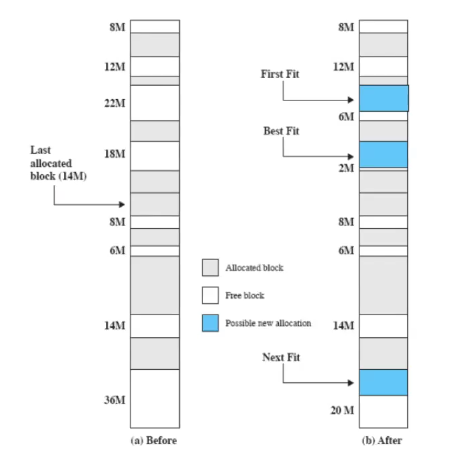
\includegraphics[width=0.75\textwidth]{immagini/AlgoritmiPartizionamento}
        \caption{Confronto tra algoritmi}
    \end{figure}

    




